\section{Background, basic approach and test site}
A multi-annual classification of aggregated crop types in Central Asia between 2000 and today based on MODIS imagery faces the following challenges:

\begin{itemize}
\item Samples and validation data are only available for some years.
\item The full extent of target classes is not known.
\item Official statistics about crops' proportions are not trustworthy.
\item The coarse geometric resolution of MODIS data is related to mixed pixel information and can lead to classification inaccuracies.
\end{itemize}

Consequently, a crucial bottleneck for a aggregated crop type classification is the lack of mapped training and validation information in most years and regions. Thus, the classification approach is not based on mapped samples. Instead, we assume 
that aggregated crop types can be characterized so called "pure samples". They represent expert knowledge formalized as $NDVI$ temporal profiles, which are considered as typical for aggregated crop types. The actual classification procedure can be distinguished into three principle steps (Fig. \ref{fig:workflow}):

\begin{enumerate}
\item MODIS pixel polygons are considered as reference units. They are coupled with raster-based MODIS $NDVI$ time series for specific years and regions as well with a preclassified irrigation mask by zonal statistics operations (ZS). 
\item Every single resulting pixel-specific MODIS $NDVI$ profile is compared with pure sample profiles by a dissimilarity test. The resulting dissimilarity matrix is used for the derivation of crop type-specific samples (SL).
\item The training samples go into a data mining procedure. A statistical model is set up between samples and MODIS $NDVI$ profiles. The model is applied on the total MODIS $NDVI$ data set predicting aggregated crop types.
\end{enumerate}

There are three options to validate the classification results with independent information. These algorithms  are not part of the classification process chain and are related to the data types \textit{points}, \textit{polygons} and \textit{raster data}.\

In the following sections, all relevant functions for classification (Sec. \ref{sec:class}) and validation (Sec. \ref{sec:val}) are described in detail and explained using the example of the Fergana test site (fig. \ref{fig:overview}), for which a classification of 2015 is carried out.\ 

The functions are implemented within the programming environment of \textbf{R} \citep[version 3.5.1; ][]{R2017}. All \textbf{R} srcipts are documented on two GitHub repositories:

\begin{itemize}
\item \texttt{CAWaClass}\footnote{\url{https://github.com/terrasys/CAWaClass.git}} collects scripts for MODIS classification.
\item \texttt{CAWaVal}\footnote{\url{https://github.com/terrasys/CAWaVal.git}} offers two options to validate a \texttt{CAWaClass} classification result.
\end{itemize}


\begin{figure}[p]
\centering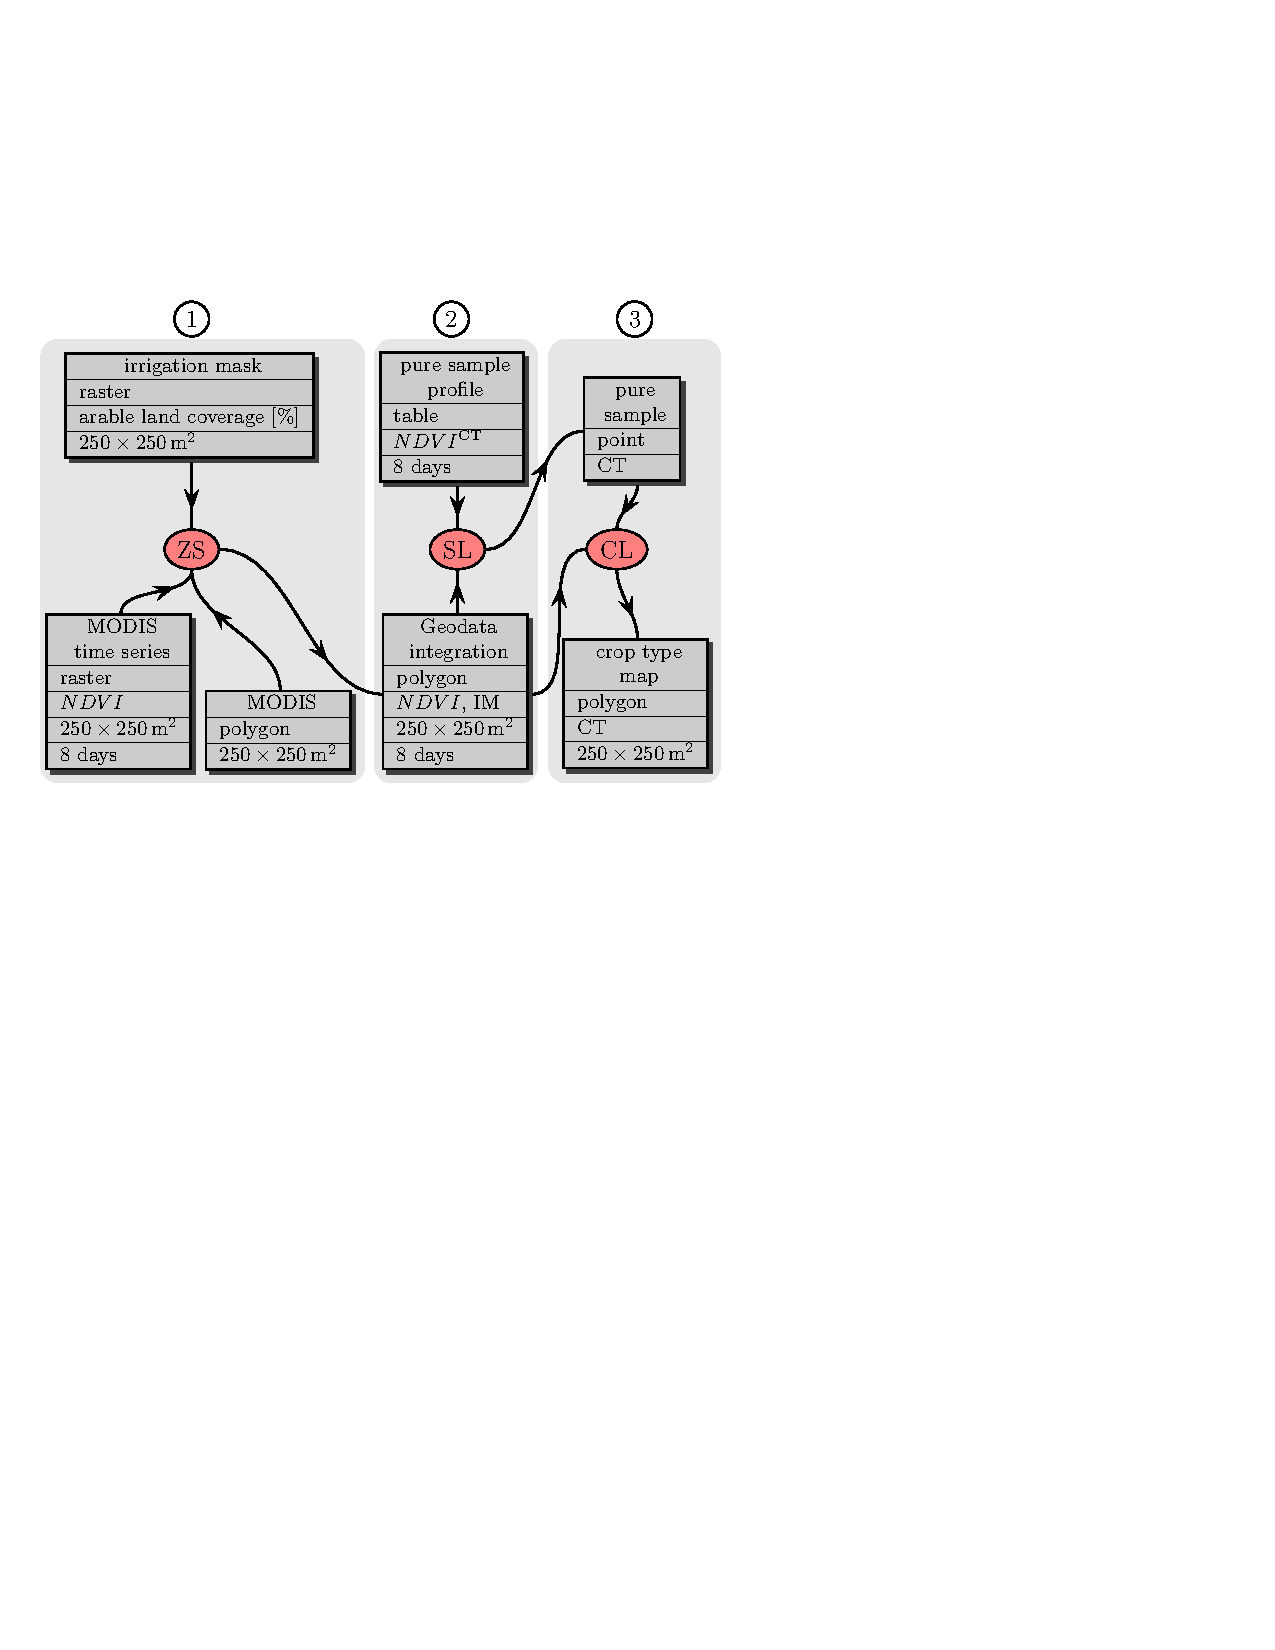
\includegraphics[width=0.8\textwidth]{figures/CaWA_workflow.pdf}
\caption{Principle workflow for the sample derivation and classification. OL -- overlay $|$ SL -- sampling $|$ ZS -- zonal statistics $|$ CT -- (aggregated) crop type  $|$ CL -- classifiation.}\label{fig:workflow}
\end{figure}

\begin{figure}[p]
\centering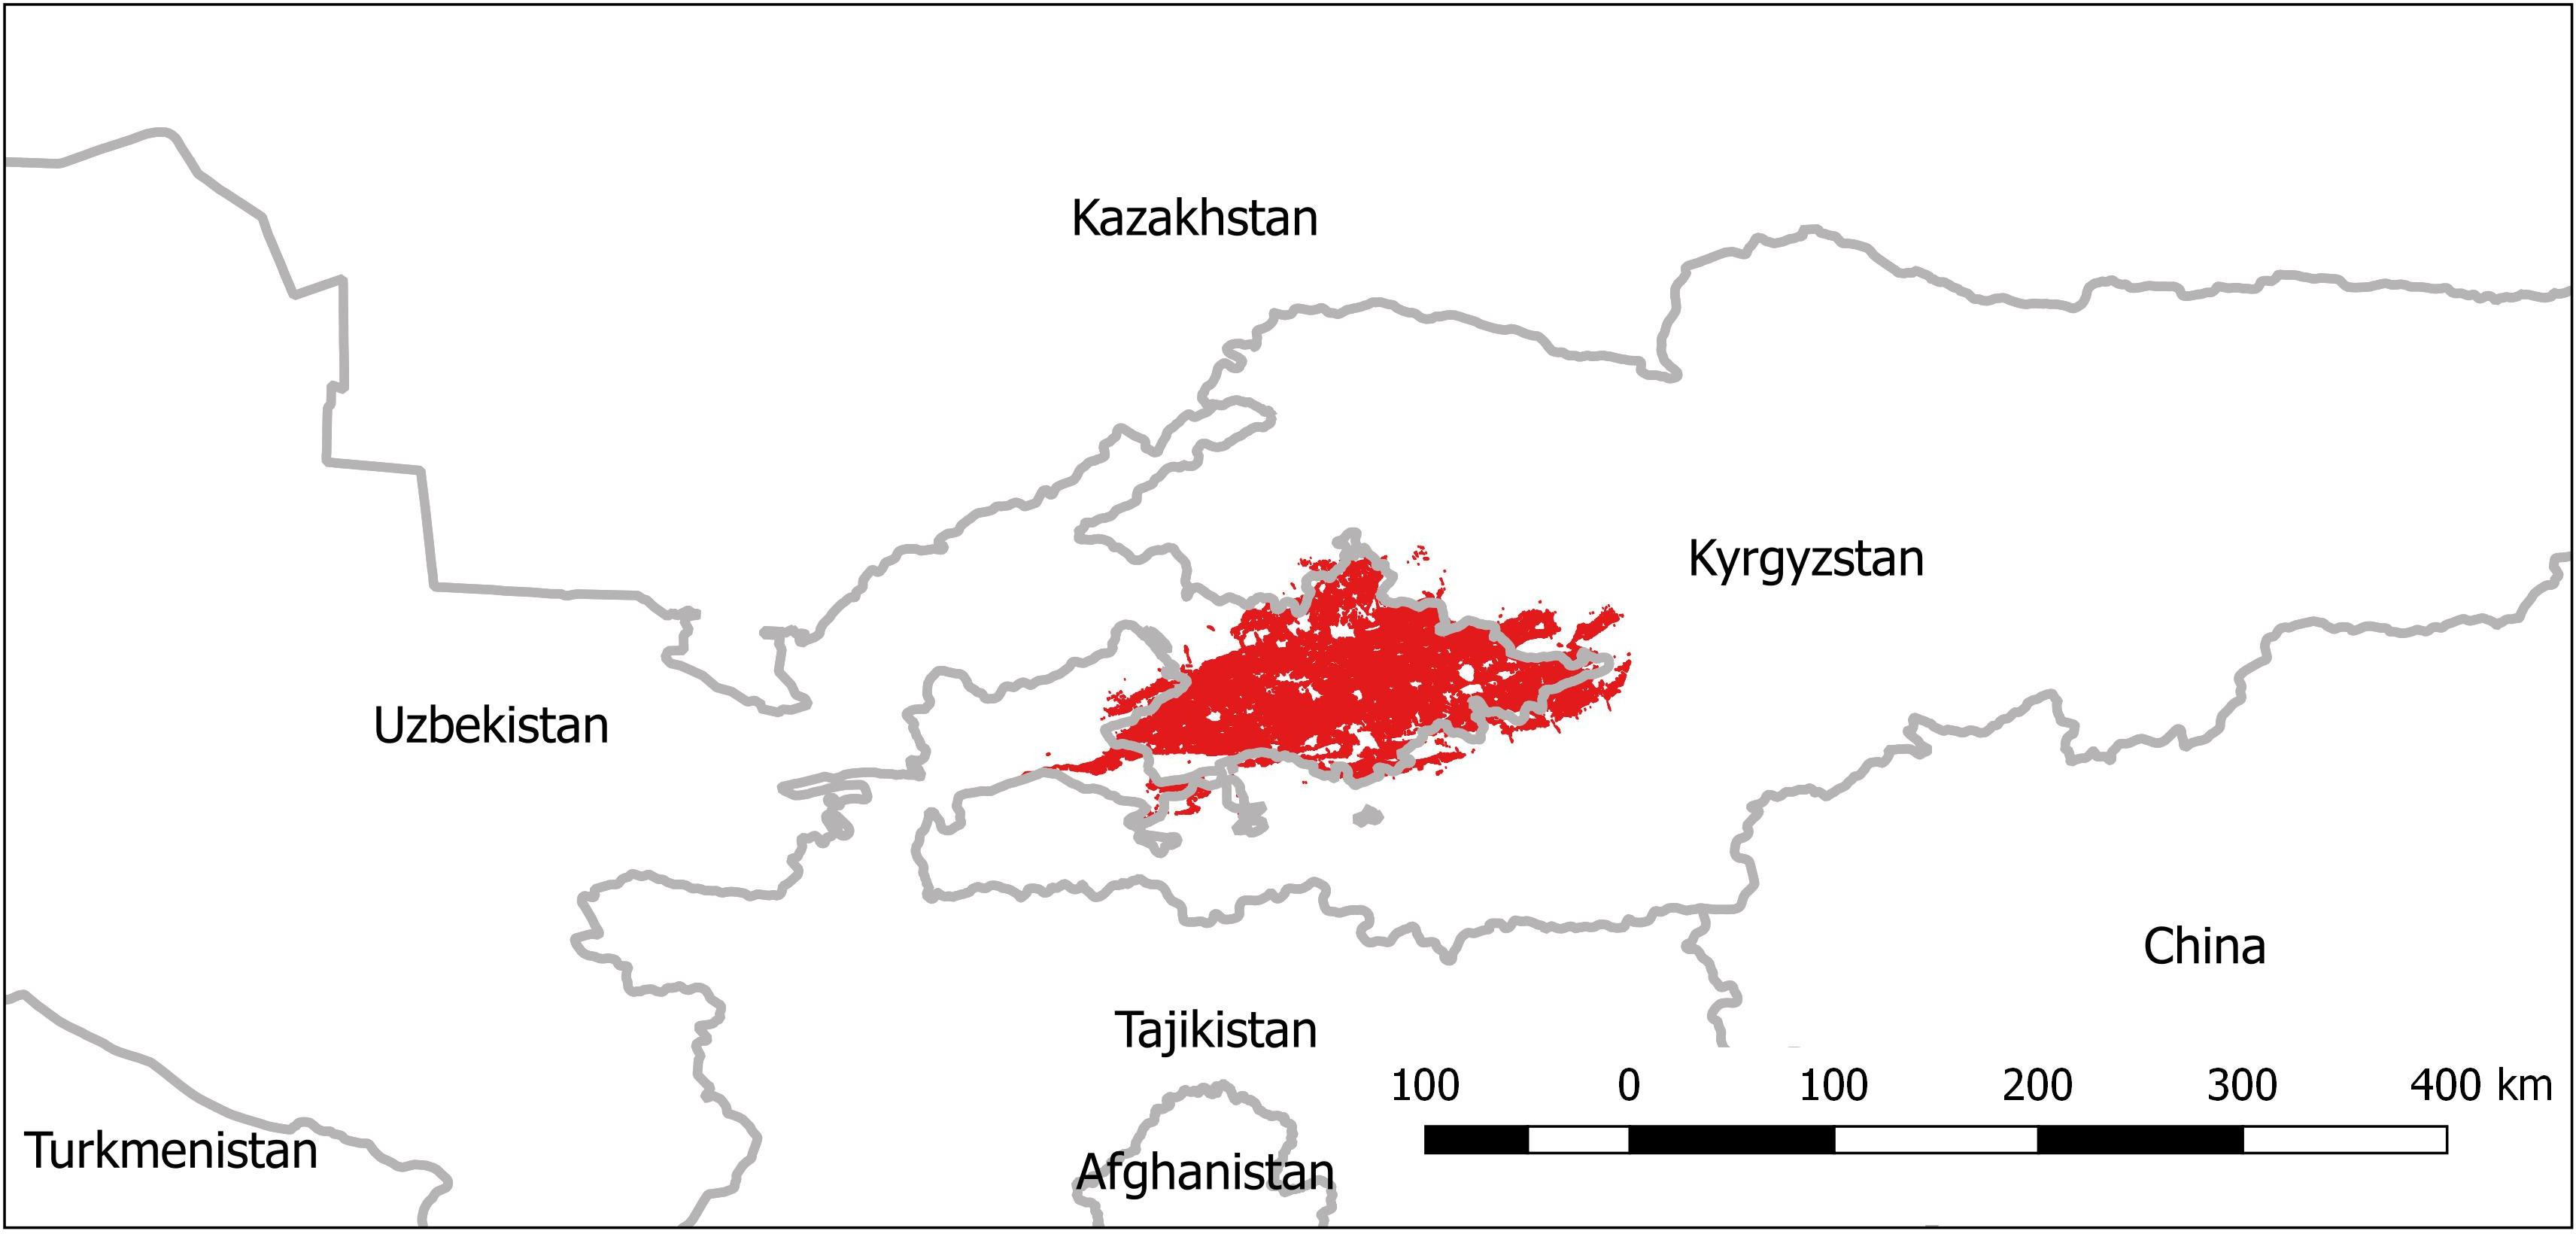
\includegraphics[width=1\textwidth]{figures/overview}
\caption{Location of the Fergana test site.}\label{fig:overview}
\end{figure}


\section{Functions}
\subsection{Classification}\label{sec:class}
All functions, which are related to classifications, are imported, parameterized and carried out by a wrapper file \texttt{callFunctions.R}. There, global settings have to be made concerning working directories or sub-folders storing input and output data (tab. \ref{tab:callFunctions}). Figure \ref{fig:cawaclass-functions} illustrates the relations between the seven functions, which are explained in detail in the following paragraphs.

\begin{table}[t]
  \centering
  \caption{Global parameters to be set in \texttt{callFunctions.R}.}
    %\begin{tabularx}{\textwidth}{X|X}
    \begin{tabular7}{ll}\toprule
    \textbf{Parameter} & \textbf{Meaning} \\\midrule
    $W.DIR$ & working directory\\\midrule
    $FUNC.DIR$ & directory containing functions \\\midrule
    $IN.DIR$ & directory containing input data \\\midrule
    $OUT.DIR$ & directory containing results \\\midrule
    $MODIS.SHP$ & name of polygon shapefile containing reference units \\\midrule
    $IM.GRD$ & name of the irrigation mask raster\\\midrule
    $PS$ & name of the text file containing pure sample $NDVI$ profiles\\ \midrule
    $YEAR$  & year of classification \\
    \bottomrule
    \end{tabular7}
    %\end{tabularx}%
  \label{tab:callFunctions}%
\end{table}


\begin{figure}[t]
\centering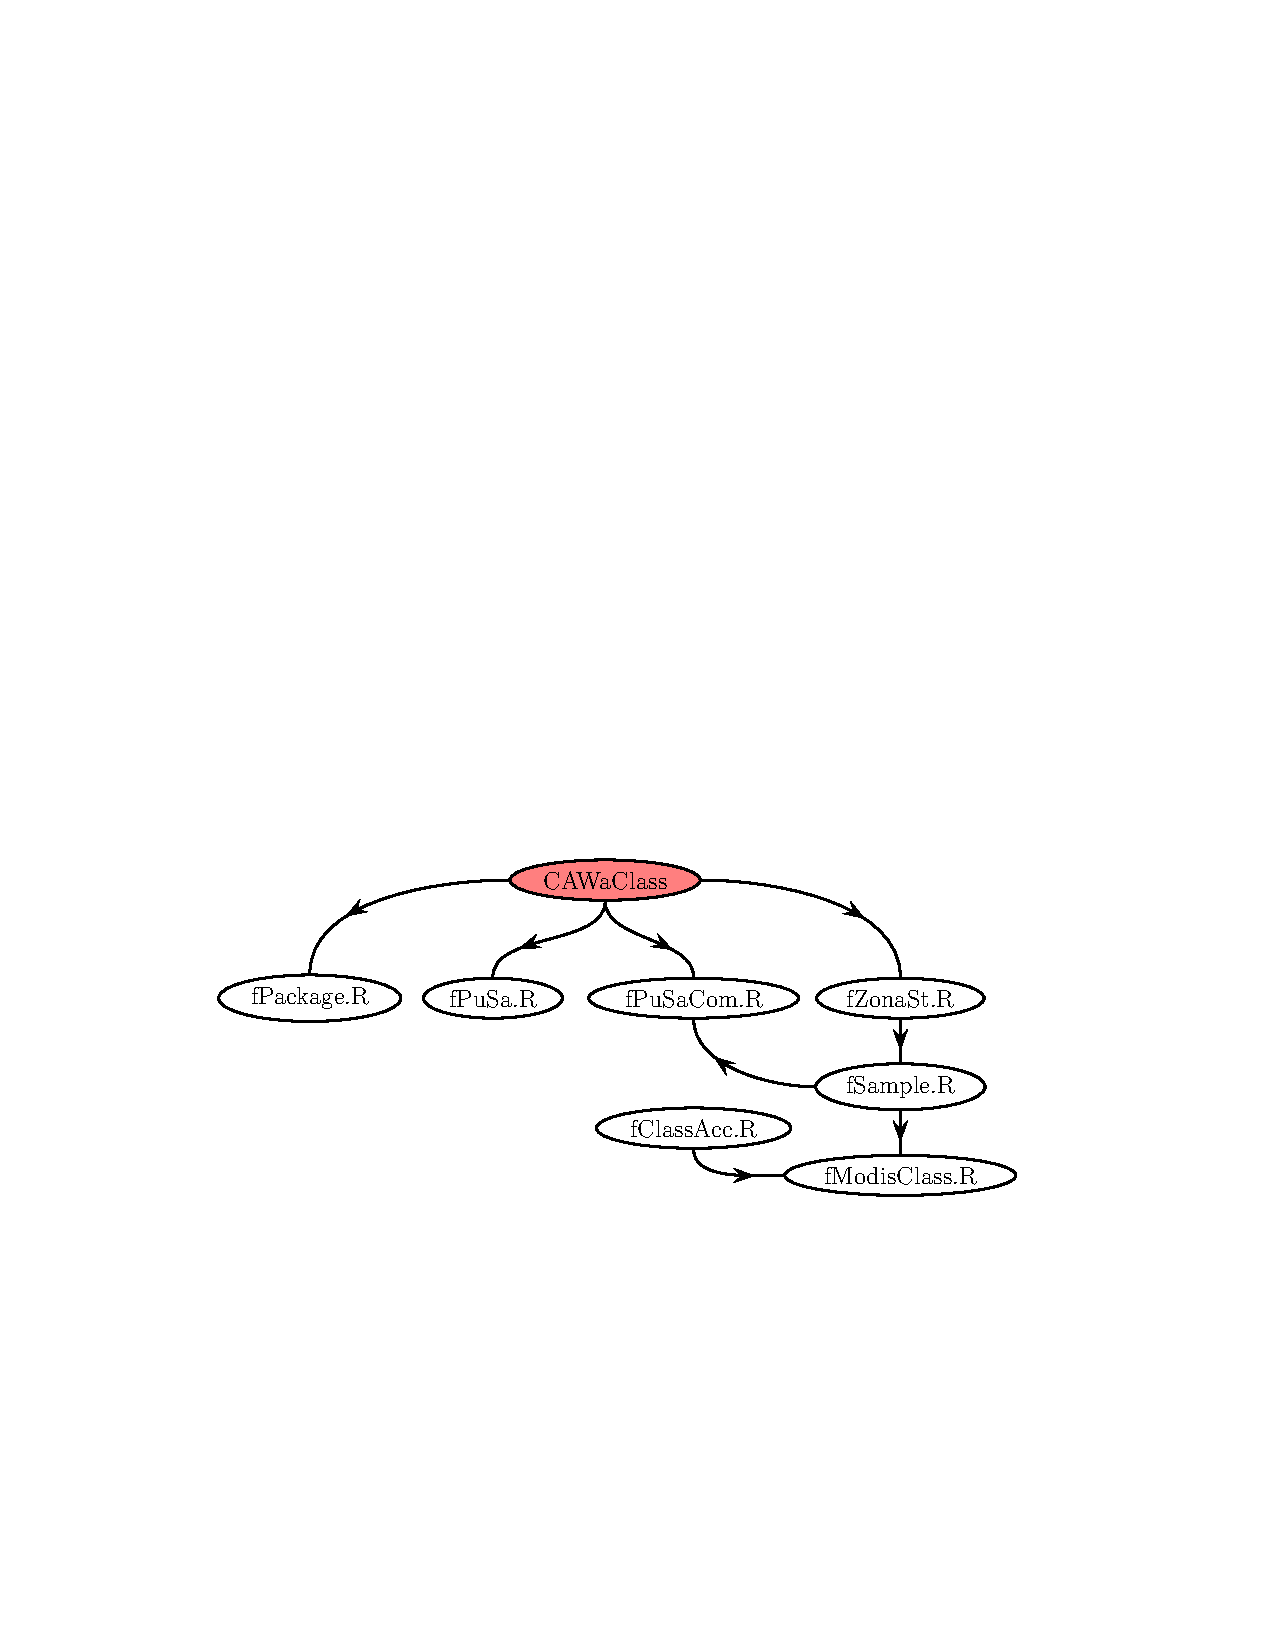
\includegraphics[width=0.75\textwidth]{figures/CAWaClass_functions.pdf}
\caption{Relations between \texttt{CAWaClass} functions.}\label{fig:cawaclass-functions}
\end{figure}

\subsubsection{fPackage}\label{sec:fPackage}
\texttt{fPackage} contains the function \texttt{loadandinstall()} for an automatic  download and installation of all required packages. In addition, the function \texttt{rsaga.env()} sets up a RSAGA geoprocessing environment \citep{Brenning2008rsaga} referring to a pre-installed SAGA-GIS version\footnote{\url{https://sourceforge.net/projects/saga-gis/files/SAGA\%20-\%202/SAGA\%202.2.2}} \citep{Conrad-etal2015gmd}.

\subsubsection{fPuSA}\label{sec:fPuSA}
The function \texttt{fPuSA()} aims at the comparison of crop type-specific $NDVI$ time series (tab. \ref{tab:fPuSa}). The comparison is based on  two functions of the  \texttt{TSclust} package, which contains measures of dissimilarity between time series \citep{MonteroVilar2014jss}:

\begin{itemize}
\item The function \texttt{diss.COR()} \say{computes dissimilarities based on the estimated Pearson's correlation of two given time series} ($d^{COR}$).
\item The function  \texttt{diss.CORT()} \say{computes an adaptive dissimilarity index between two time series that covers both dissimilarity on raw values and dissimilarity on temporal correlation behaviors} ($d^{COR}$).
\end{itemize}

Both metrics are combined by creating a scaled product $D$ resulting in a value range between 0 and 1 (Eq. \eqref{eq:d} and \eqref{eq:D}). Low $D$ values stand for a high degree of similarity, and high $D$ values for a high degree of dissimilarity.

\begin{equation}\label{eq:d}
    d = d^{COR} \times d^{CORT}
\end{equation}

\begin{equation}\label{eq:D}
    D=\dfrac{d - d_{min}}{d_{max} - d_{min}}
\end{equation}


\begin{table}[t]
  \centering
  \caption{\texttt{fPuSa}: parameters and results.}
    %\begin{tabularx}{\textwidth}{X|X}
    \begin{tabular7}{m{6.5cm}m{6.5cm}}
    \toprule
    \textbf{Parameters/results} & \textbf{Meaning} \\
    \midrule
    W.DIR & working directory \\ \midrule
    IN.DIR & directory storing input data \\ \midrule
    OUT.DIR & directory storing results \\ \midrule
    PS    & \texttt{csv}-file with class-specific $NDVI$ profiles \\ \midrule
    CLASS.NAME & name of column with class names \\ \midrule
    \midrule
    $[W.DIR]/[OUT.DIR]/[PS]$\_DM.csv & dissimilarity matrix (tab. \ref{tab:fPuSa-DM})\\ \midrule
    $[W.DIR]/[OUT.DIR]/[PS]$\_NDVI-profiles.pdf & $NDVI$ profile plot (fig. \ref{fig:ps})\\
    \bottomrule
    %\end{tabularx}%
    \end{tabular7}
  \label{tab:fPuSa}%
\end{table}

For the study region, pure samples have been used, which were generated by \citet{Conrad-etal2011ijrs}. Figure \ref{fig:ps} displays $NDVI$ profiles of five aggregated crop types. Table \ref{tab:fPuSa-DM} shows the resulting dissimilarity metrics. For instance, the $NDVI$ profiles of the classes \say{summer crop} and \say{perennial crop} are characterized by a higher similarity ($D=0,15$) than \say{summer crop}  and \say{winter crop} ($D=0,67$). 

\begin{figure}[p]
\centering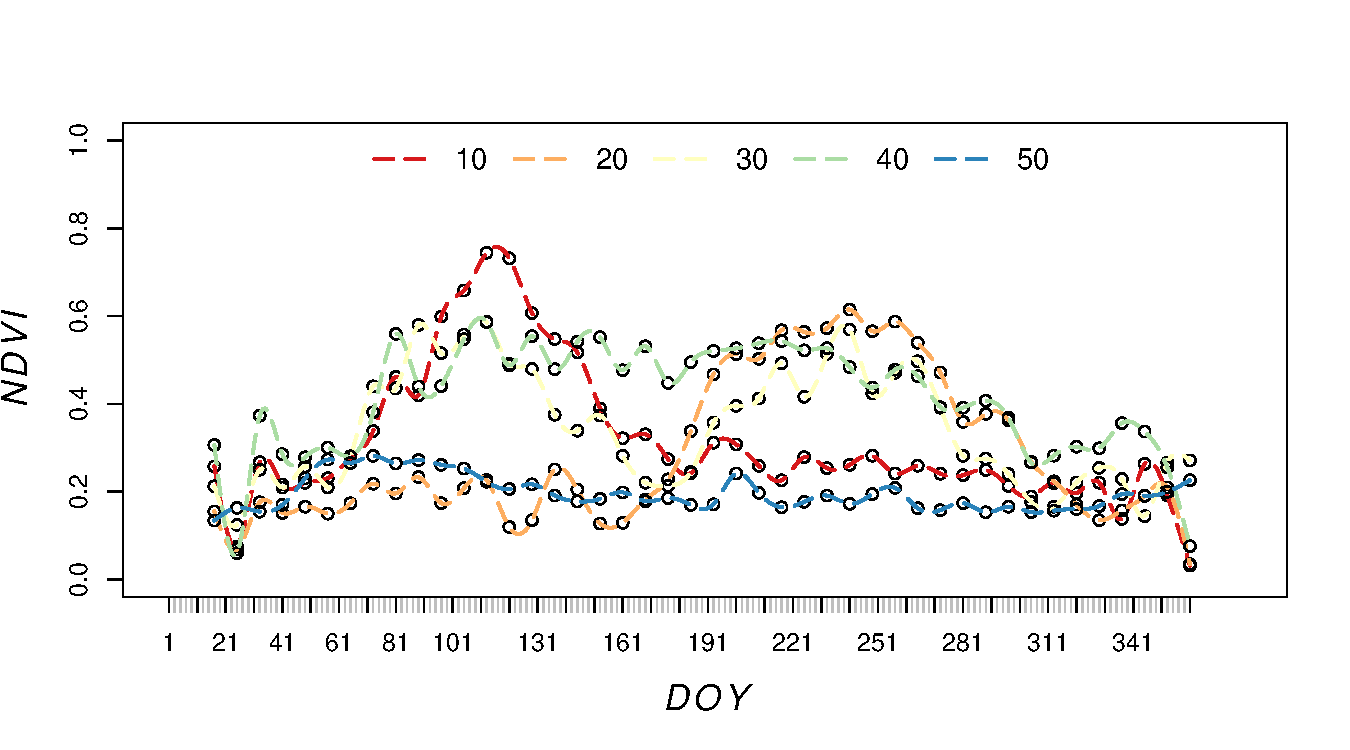
\includegraphics[width=1\textwidth]{figures/PureSample_NDVI-profiles}
\caption{\texttt{fPuSa} output: $NDVI$ profiles of aggregated crop types derived from samples and MODIS imagery according to \citet{Conrad-etal2011ijrs}. 10 -- summer crop $|$ 20 -- winter crop $|$ 30 -- double crop $|$ 40 -- perennial Crop $|$ 50 -- bare land.}\label{fig:ps}
\end{figure}

\begin{table}[p]
  \centering
  \caption{\texttt{fPuSa.R} output: matrix of class-specific dissimilarity values ($D^{[10,20,30,40,50]}$). 10 -- summer crop $|$ 20 -- winter crop $|$ 30 -- double crop $|$ 40 -- perennial crop $|$ 50 -- bare land.}
    \begin{tabular7}{r|r|r|r|r|r}
    \toprule
    & $D^{10}$ & $D^{20}$ & $D^{30}$ & $D^{40}$ & $D^{50}$ \\
    \midrule
    $D^{10}$ & 0,00  & 0,67  & 0,25  & 0,15  & 0,66 \\
    \midrule
    $D^{20}$ & 0,67  & 0,00  & 0,26  & 0,31  & 0,89 \\
    \midrule
    $D^{30}$ & 0,25  & 0,26  & 0,00  & 0,17  & 0,53 \\
    \midrule
    $D^{40}$ & 0,15  & 0,31  & 0,17  & 0,00  & 1,00 \\
    \midrule
    $D^{50}$ & 0,66  & 0,89  & 0,53  & 1,00  & 0,00 \\
    \bottomrule
    \end{tabular7}%
  \label{tab:fPuSa-DM}%
\end{table}%

\subsubsection{fZonaSt}\label{sec:ZonaSt}
The function \texttt{fZonaSt()} enables a coupling of arbitrary reference units with both MODIS $NDVI$ raster files for any year or region ([YEAR]-[MONTH]-[DAY]\_ndvi.tif) and a predefined irrigation mask raster file (tab. \ref{tab:fZonaSt}). The actual coupling  procedure is realized by using the RSAGA function   \texttt{rsaga.geoprocessor()}, which allows the execution of SAGA-GIS modules. The zonal statistics algorithm can be found in the library \texttt{shapes\_grid}, where module 2 is related to the corresponding zonal statistics function. As a result, the reference units shape file is parametrized by a irrigation mask value ($IM \in [0,128]$) and DOY-specific $NDVI$ values $(MD[DOY] \in [0,1]$).  The extent of the irrigation mask includes the total area in Central Asia, which should be classified. Here, an irrigation mask threshold of $V.IM=100$  is used for the selection of irrigation areas in the Fergana test site.

\begin{table}[pt]
  \centering
  \caption{\texttt{fZonaSt}: parameters and results.}
    \begin{tabular7}{m{6.5cm}m{6.5cm}}\toprule
    %\begin{tabularx}{\textwidth}{X|X}
    \textbf{Parameters/results} & \textbf{Meaning} \\\midrule
    W.DIR & working directory \\ \midrule
    IN.DIR & directory storing input data \\ \midrule
    OUT.DIR & directory storing results \\ \midrule
    MODIS.SHP    & name of reference unit shapefile [*.shp]\\ \midrule
    IM.GRD & name of irrigation mask raster file [*.sgrd]\\ \midrule
    V.IM & threshold for selecting the irrigation area\\ \midrule
    YEAR & year to be classified\\ \midrule
    \midrule
    $[W.DIR]/[OUT.DIR]/$ $[MODIS.SHP,YEAR]$.shp & shape file with a irrigation mask value ($IM \in [0,100]$) as well as $NDVI$ values for specific years and DOYs ($MD[DOY] \in [0,1]$)\\
    \bottomrule
    %\end{tabularx}
    \end{tabular7}
  \label{tab:fZonaSt}%
\end{table}

\begin{table}[htp]
  \centering
  \caption{\texttt{fSample}: parameters and results.}
    \begin{tabular7}{m{6.5cm}m{6.5cm}}
    %\begin{tabularx}{\textwidth}{X|X}
    \toprule
    \textbf{Parameters/results} & \textbf{Meaning} \\
    \midrule
    W.DIR & working directory \\ \midrule
    IN.DIR & directory storing input data \\ \midrule
    OUT.DIR & directory storing results \\ \midrule
    PS    & \texttt{csv}-file with class-specific $NDVI$ profiles\\ \midrule
    MODIS.SHP    & name of reference unit shapefile [*.shp]\\ \midrule
    ZS.SHP & shape file with $NDVI$ values for specific DOYs and YEARs; result from \texttt{fZonaSt()} function\\ \midrule
    Q & quantile of $D$ value distribution (Sec. \ref{sec:fPuSA})\\
    \midrule \midrule
     $[W.DIR]/[OUT.DIR]/$ $[MODIS.SHP,YEAR]$\_SAMPLE-NDVI-densityplot\_Q[Q].pdf & density plot of class-  and  pixel-specific  dissimiliarity  values (tab. \ref{tab:fSample-DM} and fig. \ref{fig:fSample-density})\\ \midrule
     $[W.DIR]/[OUT.DIR]/$ $[MODIS.SHP,YEAR]$\_SAMPLE-NDVI-barplot\_Q[Q].pdf & barplot of class-specific samples\\ \midrule
    $[W.DIR]/[OUT.DIR]/$ $[MODIS.SHP,YEAR]$\_DM.csv & class-  and  pixel-specific  dissimiliarity  matrix (tab. \ref{tab:fSample-DM})\\ \midrule
    $[W.DIR]/[OUT.DIR]/$ $[MODIS.SHP,YEAR]$.shp & sample shape file with an irrigation mask value ($IM \in [0,100]$) as well as $NDVI$ values for specific years and DOYs ($MD[DOY] \in [0,1]$)\\ \midrule
    $[MODIS.SHP,YEAR]$\_SAMPLE-NDVI\_agg\_Q[Q].csv & aggregated samples of class-specific $NDVI$ values\\
    \bottomrule
    %\end{tabularx}%
    \end{tabular7}
  \label{tab:fSample}%
\end{table}


\subsubsection{fSample}\label{sec:fSample}
The function \texttt{fSample()} aims at the localization of samples for specific years and sites (tab. \ref{tab:fSample}). The procedure is based on the dissimilarity test introduced in section \ref{sec:fPuSA} and can be structured into two steps:

\begin{enumerate}
\item Comparison of pure sample $NDVI$ profiles (parameter PS) with pixel-sepecific MODIS $NDVI$ profiles (parameter ZS.SHP) by applying the functions \texttt{diss.COR} and \texttt{diss.CORT} and calculation of class- and pixel-specific $D$ values (Sec. \ref{sec:fPuSA}), 
\item Calculation of class-specific quantiles of $D$ value distributions and selection of pixels, which fulfill a user-specific quantile-based thresholds (parameter $Q$) and removing duplicates.
\end{enumerate}

In table \ref{tab:fSample-DM}, a subset of  class- and pixel-specific dissimilarity values ($D^{[10,20,30,40,50]}$) is shown. The corresponding class-specfic density functions are displayed in figure \ref{fig:fSample-density}. The red dashed vertical lines mark the position of user-specific quantiles, which act as dynamic thresholds for sample selection. The selection result can be controlled using figure  \ref{fig:fSample-barplot}, where the sample number and the class-specific sample proportions are displayed. Accordingly, for 2015 a total sample number of 9587 could be selected. The sample class proportions are nearly equal, which is related to the quantile-based selection approach. 




% Table generated by Excel2LaTeX from sheet 'Sheet1'
\begin{table}[tp]
  \centering
  \caption{\texttt{fSample.R} output: subset of class- and pixel-specific dissimilarity values ($D^{[10,20,30,40,50]}$). ID -- MODIS pixel ID $|$  10 -- summer crop $|$ 20 -- winter crop $|$ 30 -- double crop $|$ 40 -- perennial crop $|$ 50 -- bare land.} \label{tab:fSample-DM}
    \begin{tabular7}{r|r|r|r|r|r}\toprule
    ID & $D^{10}$    & $D^{20}$    & $D^{30}$    & $D^{40}$    & $D^{50}$ \\\midrule
    316   & 0,28  & 0,52  & 0,38  & 0,13  & 0,43 \\
    317   & 0,24  & 0,50  & 0,35  & 0,14  & 0,38 \\
    318   & 0,22  & 0,60  & 0,40  & 0,17  & 0,31 \\
    319   & 0,25  & 0,54  & 0,36  & 0,19  & 0,43 \\
    1374  & 0,22  & 0,67  & 0,44  & 0,17  & 0,44 \\
    1375  & 0,21  & 0,63  & 0,38  & 0,17  & 0,38 \\
    1376  & 0,22  & 0,66  & 0,41  & 0,17  & 0,39 \\
    2425  & 0,27  & 0,42  & 0,27  & 0,13  & 0,53 \\
    2426  & 0,26  & 0,56  & 0,33  & 0,15  & 0,42 \\
    2427  & 0,20  & 0,60  & 0,43  & 0,15  & 0,41 \\
    $\dots$ & $\dots$ & $\dots$&$\dots$   &$\dots$ & $\dots$\\\bottomrule
    \end{tabular7}%
\end{table}%

\begin{figure}[p]
    \centering
\subfigure[summer crop (10)]{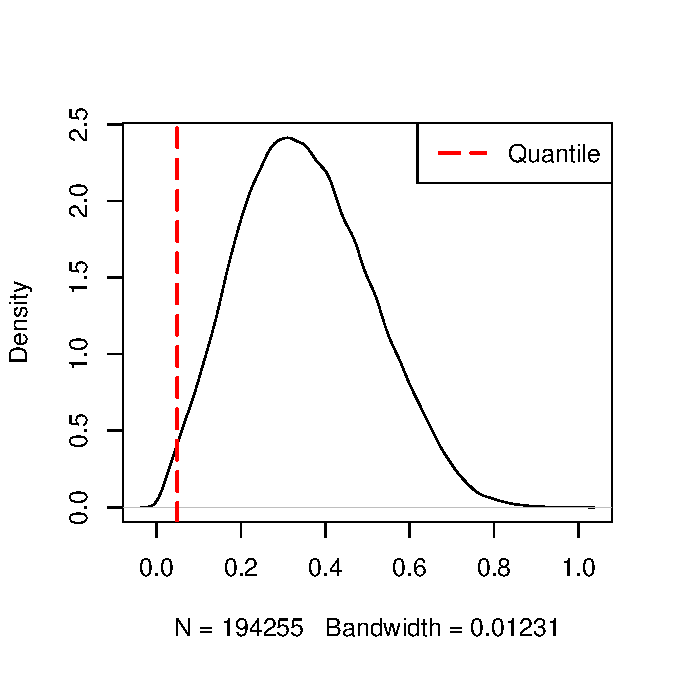
\includegraphics[width=0.45\textwidth]{figures/MODIS_fergana2015_SAMPLE-NDVI-densityplot_Q1_Part1.pdf}}
\subfigure[winter crop (20)]{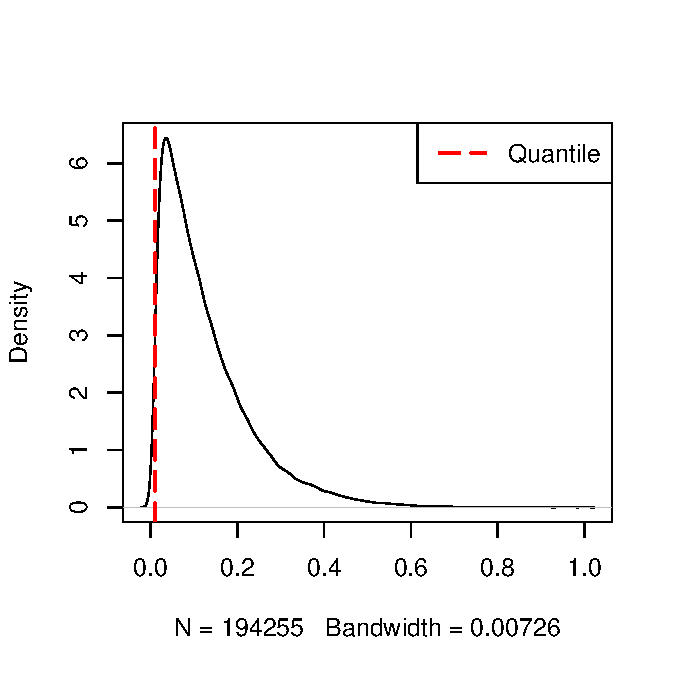
\includegraphics[width=0.45\textwidth]{figures/MODIS_fergana2015_SAMPLE-NDVI-densityplot_Q1_Part2.pdf}}

\subfigure[double crop (30)]{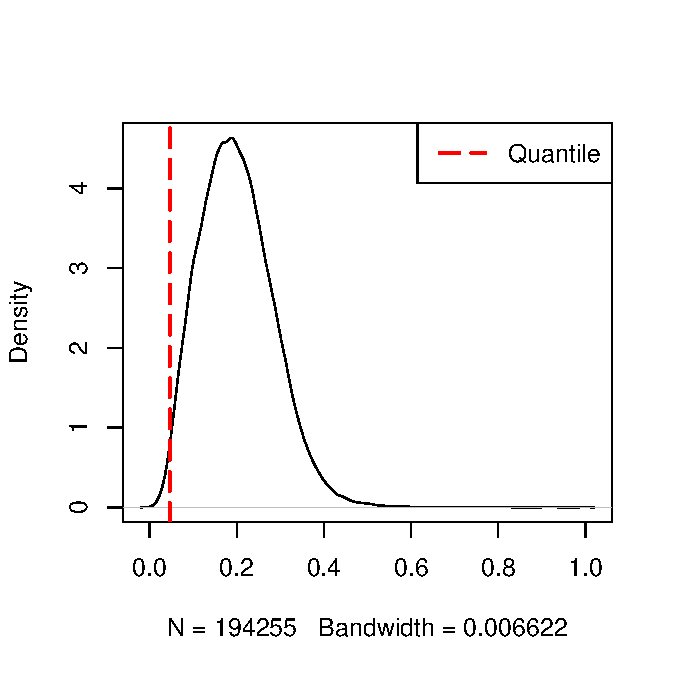
\includegraphics[width=0.45\textwidth]{figures/MODIS_fergana2015_SAMPLE-NDVI-densityplot_Q1_Part3.pdf}}
\subfigure[perennial crop (40)]{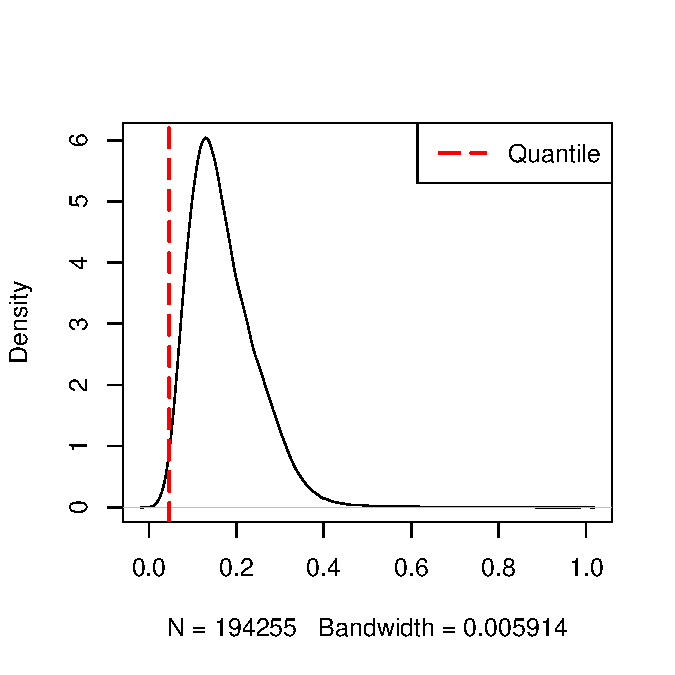
\includegraphics[width=0.45\textwidth]{figures/MODIS_fergana2015_SAMPLE-NDVI-densityplot_Q1_Part4.pdf}}

\subfigure[bare land (50)]{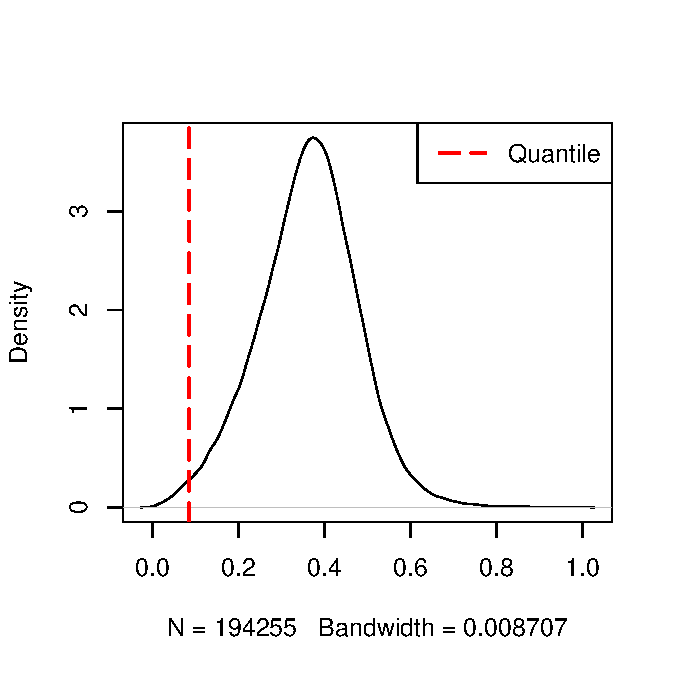
\includegraphics[width=0.45\textwidth]{figures/MODIS_fergana2015_SAMPLE-NDVI-densityplot_Q1_Part5.pdf}}
    \caption{\texttt{fSample} output: Density plots of class-  and  pixel-specific  dissimiliarity  values (see tab. \ref{tab:fSample-DM}).}
    \label{fig:fSample-density}
\end{figure}

\begin{figure}[H]
\centering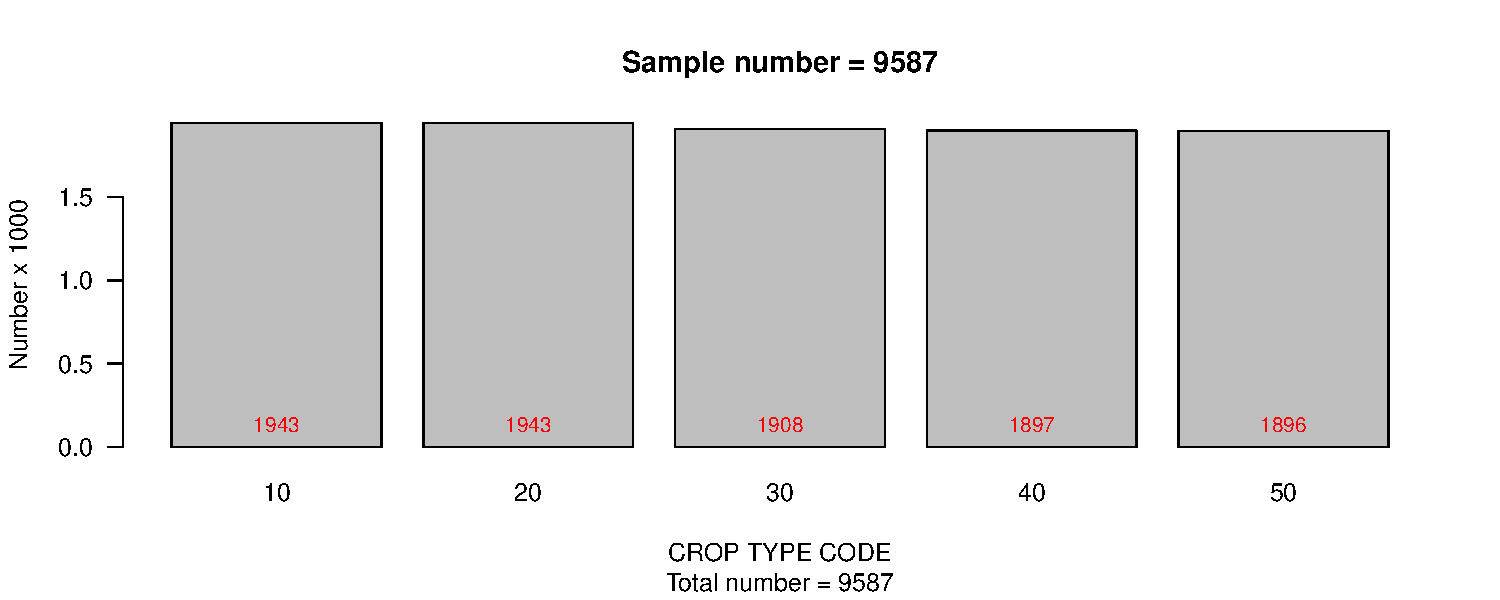
\includegraphics[width=1\textwidth]{figures/MODIS_fergana2015_SAMPLE-NDVI-barplot_Q1.pdf}
\caption{\texttt{fSample} output: barplot of class-specific samples. 10 -- summer crop $|$ 20 -- winter crop $|$ 30 -- double crop $|$ 40 -- perennial Crop $|$ 50 -- bare land.}\label{fig:fSample-barplot}
\end{figure}

\begin{table}[H]
  \centering
  \caption{\texttt{fPuSaCom}: parameters and results.}
    %\begin{tabularx}{\textwidth}{X|X}
    \begin{tabular7}{m{6.5cm}m{6.5cm}}
    \toprule
    \textbf{Parameters/results} & \textbf{Meaning} \\
    \midrule
    W.DIR & working directory \\ \midrule
    IN.DIR & directory storing input data \\ \midrule
    OUT.DIR & directory storing results \\ \midrule
    CLASS.NAME & name of column with class names\\ \midrule
    PS1 & \texttt{csv}-file with class-specific $NDVI$ profiles\\ \midrule
    PS2 & \texttt{csv}-file with aggregated class-specific $NDVI$ profiles derived from applying funtion \texttt{fSample()}\\ \midrule
    PS1PF & name prefix in column name of PS1\\ \midrule
    PS2PF & name prefix in column name of PS2\\ \midrule
    \midrule
    $[W.DIR]/[OUT.DIR]/$ $[PS1]\_\_[PS2]$.pdf &  plot of class-specific $NDVI$ profiles based on both pure samples and aggregated samples derived with \texttt{fSample()} function\\
    \bottomrule
    %\end{tabularx}%
    \end{tabular7}
  \label{tab:fPuSaCom}%
\end{table}


\begin{figure}[t]
\centering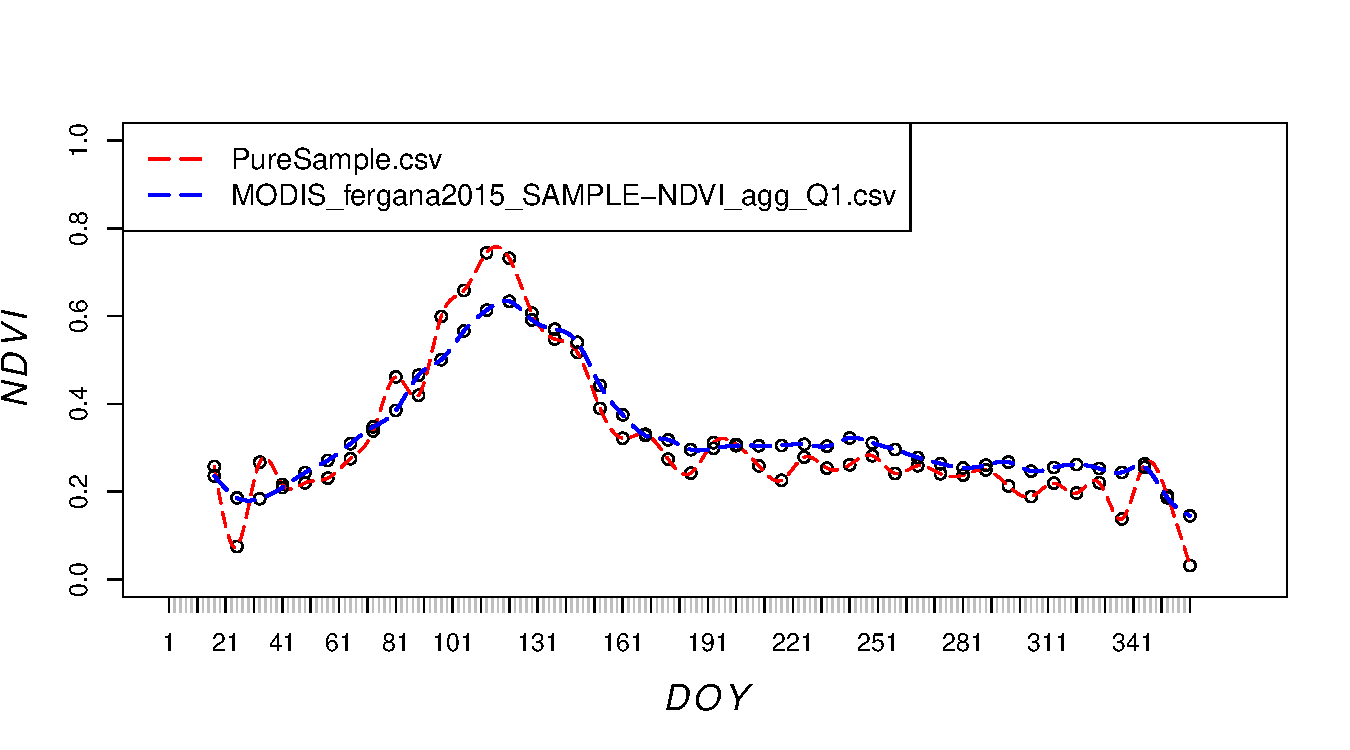
\includegraphics[width=1\textwidth]{figures/PureSample__MODIS_fergana2015_SAMPLE-NDVI_agg_Q1_Part1.pdf}
\caption{\texttt{fPuSaCom} output: plot of class-specific $NDVI$ profiles based on both pure samples and aggregated samples derived with \texttt{fSample()} function on the example of land use class 10 (summer crops).}\label{fig:fPuSaCom}
\end{figure}

\subsubsection{fPuSaCom}
Function \texttt{fPuSaCom()} enables the comparison of pure samples (Sec. \ref{sec:fPuSA}) and aggregated samples derived with function \texttt{fSample()} (Sec. \ref{sec:fSample}). As a result,  comparing plots of class-specific $NDVI$ profiles are generated. As shown in figure \ref{fig:fPuSaCom} on the example of class \say{summer crops}, the profiles can be visually assessed regarding their similarity.

\subsubsection{fModisClass \& fClassAcc}\label{sec:fModisClass}
The test site- and year-specific classification is realized by executing the function \texttt{fModis}- \texttt{Class()} (tab. \ref{tab:fModisClass}), where some functions of the \textbf{R} package \texttt{caret} are combined \citep{KuhnJohnson2013apm,Kuhn-etal2018}. The  classification process starts with a data partition procedure (here: 75\,\% training data and 25\,\% test data) considering the class proportions (function \texttt{caret::createDataPartition}), which is applied to the sample shape file derived from the  function \texttt{fSample()} (Sec. \ref{sec:fSample}). The option \texttt{caret::upSample} enables to adapt the sample number of the minority class to the same size as the majority class.\


The function \texttt{caret::train} is used for the actual model building. There, the classifier can be set by user (option M.TRAIN)\footnote{\url{https://topepo.github.io/caret/train-models-by-tag.html}}. 
The classification of the Fergana test site is based on \say{Random Forest} (RF) algorithm, which has been proven as robust classifier for remore sensing applications \citep{BelgiuDragut2016jprs}. RF is  representative of data mining algorithms and stands for a re\-gres\-si\-on- and ensemble-based decision tree algorithm. RF splits the feature space of the explanatory variables until the resulting tree shows the best statistical correlation by minimizing the variance. Based on bootstrapped samples, RF generates a large number of independent trees (ensembles). Two thirds of the samples are used for growing trees (\textit{in-bag} data), and one third are randomly drawn with a replacement for the calculation of error estimates by cross-validation  \citep[\textit{out-of-bag} data; ][]{Breiman2001ml}.\


Figure \ref{fig:fModisClass} illustrates the shape file of classified crop types and their  proportional coverage of areas. The shape file also contains information about the pixel-specific class probability, which expresses the proportion of the trees that voted for each class. Apart from that, following information about the classification accuracy are provided:



\begin{itemize}
\item The overall accuracy is based on a repeated 10-fold cross validation of the training data set and can be considered as the internal model accuracy.  
\item The fitted model is used for the classification of the test data set, for which a confusion matrix and accuracy metrics are calculated (external validation) by activating function \texttt{fClassAcc()}\footnote{\url{https://github.com/saidbleik/Evaluation/blob/master/eval.R}}.
The  \textit{F1} score represents the weighted harmonic mean of the metrics \say{precision} and \say{recall} (Eq. \eqref{eq:f-measure}). Both metrics result from the quotient of the \say{number of correctly classified instances per class} with  \say{the number of predictions per class} (Eq. \eqref{eq:precision}; precision) and {the number of instances per class} (Eq. \eqref{eq:recall}; recall), respectively.
\end{itemize}

The internal accuracy assessment for the MODIS-based classification of the Fergana test site are listed in table  \ref{tab:ModisClassCM} and \ref{tab:ModisClassAM}.

\begin{equation}
\label{eq:f-measure}
\text{F1} = 2 * \frac{\text{Precision} * \text{Recall}}{\text{Precision} + \text{Recall}}
\end{equation}

\begin{table}[H]
	\centering
	\caption{\texttt{fModisClass}: parameters and results.}
	%\begin{tabularx}{\textwidth}{X|X}
	\begin{tabular7}{m{6.5cm}m{6.5cm}}
		\toprule
		\textbf{Parameters/results} & \textbf{Meaning} \\
		\midrule
		W.DIR & working directory \\ \midrule
		IN.DIR & directory storing input data \\ \midrule
		OUT.DIR & directory storing results \\ \midrule
		ZS.SHP & shape file with $NDVI$ values for specific DOYs and YEARs; result from \texttt{fZonaSt()} function\\ \midrule
		SAMPLE.SHP & sample shape file resulting from applying function \text{fSample()}\\\midrule
		PART & proportion of SAMPLE.SHP which should be used for training [$\in 0,1$] and validation\\\midrule
		T.CLASS & name of column within SAMPLE.SHP file with target class names\\\midrule
		M.TRAIN & classification method\\\midrule
		UpSample=TRUE & randomly sample (with replacement) the minority class to be the same size as the majority class\\\midrule\midrule
		$[W.DIR]/[OUT.DIR]/$ $[SAMPLE.SHP]\_[M.TRAIN]$\_CV.txt &  cross validation result\\\midrule
		$[W.DIR]/[OUT.DIR]/$ $[SAMPLE.SHP]\_[M.TRAIN]$\_AM.csv & accuracy metrics based on test data set derived from data partition of SAMPLE.SHP\\\midrule
		$[W.DIR]/[OUT.DIR]/$ $[SAMPLE.SHP]\_[M.TRAIN]$\_CM.csv & confusion matrix based on test data set derived from data partition of SAMPLE.SHP\\\midrule
		$[W.DIR]/[OUT.DIR]/$ $[ZS.SHP]\_[M.TRAIN]$\_CLASS.shp & shape file with classification result and corresponding class probobility (columns [CLASS] and [CLASS]\_PB) \\\midrule
		$[W.DIR]/[OUT.DIR]/$ $[ZS.SHP]\_[M.TRAIN]$\_CLASS.pdf & barplot of classified crop types\\
		\bottomrule
		%\end{tabularx}%
	\end{tabular7}
	\label{tab:fModisClass}%
\end{table}

\begin{equation}
\label{eq:precision}
\text{Precision} = \frac{\text{Diag}}{\text{colsums}}
\end{equation}

\begin{equation}
\label{eq:recall}
   \text{Recall} = \frac{\text{Diag}}{\text{rowsums}} 
\end{equation}


\begin{figure}[H]
	\centering\subfigure[]{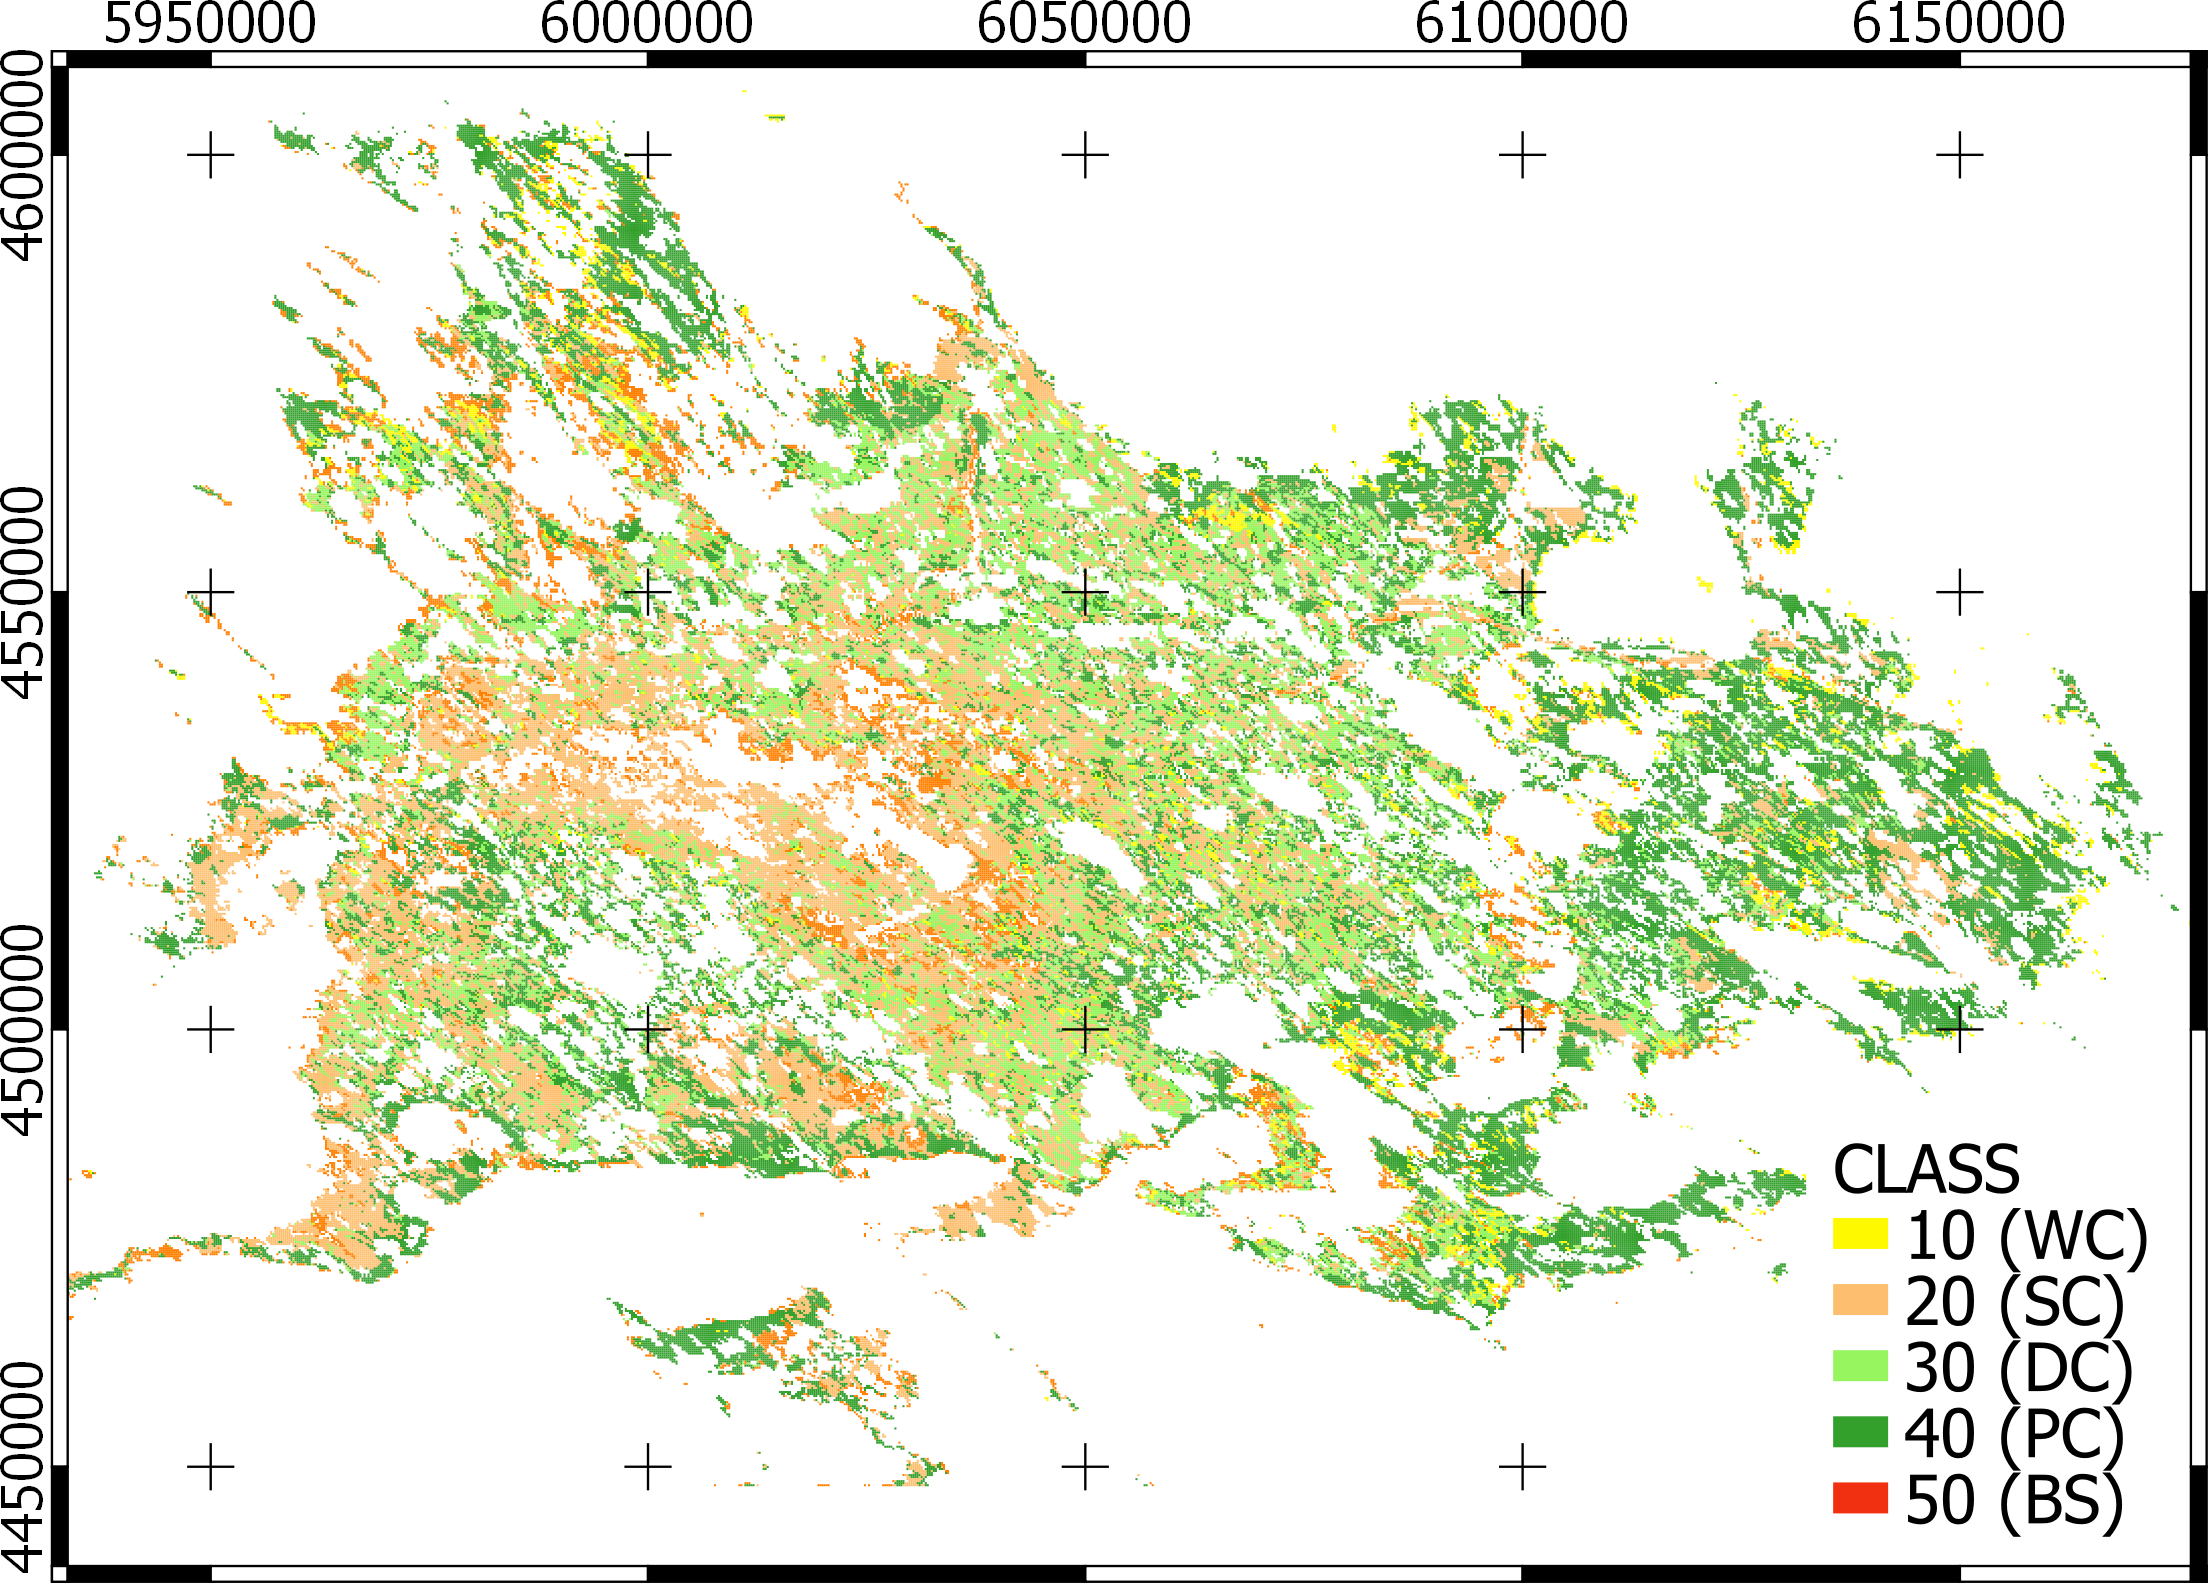
\includegraphics[width=1\textwidth]{figures/Fergana_Class2015.png}}
	\centering\subfigure[]{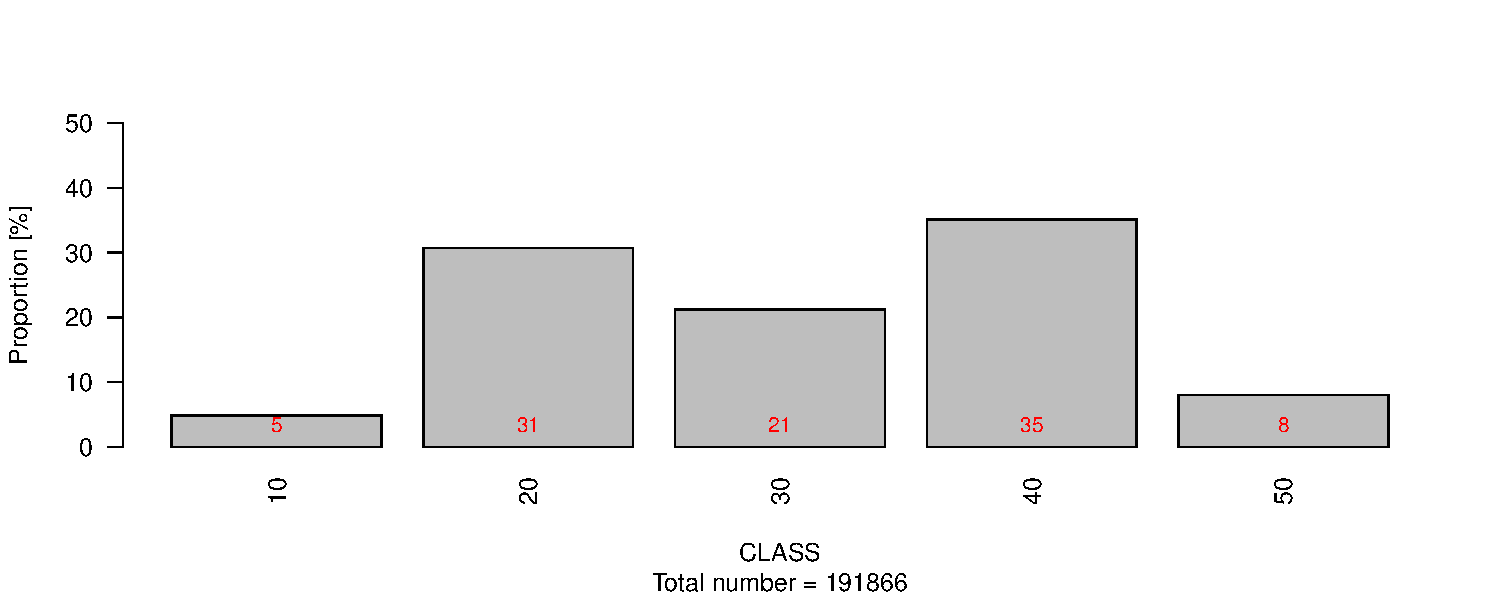
\includegraphics[width=1\textwidth]{figures/MODIS_fergana2015_rf_classification_barplot.pdf}}
	\caption{\texttt{fModisClass} output: Classification result and barplot of classified crop types on the example of Fergana test site and 2015. 10 -- summer crop $|$ 20 -- winter crop $|$ 30 -- double crop $|$ 40 -- perennial crop $|$ 50 -- bare land.}\label{fig:fModisClass}
\end{figure}


\begin{table}[t]
    \caption{\texttt{fModisClass} output: Confusion matrix based on test data set on the example of Fergana test site and 2015. 10 -- summer crop $|$ 20 -- winter crop $|$ 30 -- double crop $|$ 40 -- perennial crop $|$ 50 -- bare land.}\label{tab:ModisClassCM}
    \centering
   \begin{tabular7}{r|r|r|r|r|r}\toprule
          & \textbf{10}    & \textbf{20}    & \textbf{30}    & \textbf{40}    & \textbf{50} \\\midrule
    10    & 447   & 0     & 2     & 6     & 9 \\\midrule
    20    & 0     & 507   & 0     & 0     & 0 \\\midrule
    30    & 5     & 0     & 463   & 8     & 1 \\\midrule
    40    & 1     & 0     & 8     & 464   & 1 \\\midrule
    50    & 3     & 0     & 1     & 0     & 470 \\\bottomrule
    \end{tabular7}%
\end{table}

\begin{table}[t]
    \caption{\texttt{fModisClass} output: Accuracy metrics based on test data set on the example of Fergana test site and 2015. 10 -- summer crop $|$ 20 -- winter crop $|$ 30 -- double crop $|$ 40 -- perennial crop $|$ 50 -- bare land.}\label{tab:ModisClassAM}
    \centering
       \begin{tabular7}{r|r|r|r|r|r}\toprule
          & \textbf{10}    & \textbf{20}    & \textbf{30}    & \textbf{40}    & \textbf{50} \\\midrule
    \textbf{Accuracy} & 0,98  & 0,98  & 0,98  & 0,98  & 0,98 \\\midrule
    \textbf{Precision} & 0,98  & 1,00  & 0,98  & 0,97  & 0,98 \\\midrule
    \textbf{Recall} & 0,96  & 1,00  & 0,97  & 0,98  & 0,99 \\\midrule
    \textbf{F1}    & 0,97  & 1,00  & 0,97  & 0,97  & 0,98 \\\midrule
    \textbf{Kappa} & 0,98  & 0,98  & 0,98  & 0,98  & 0,98 \\\bottomrule
    \end{tabular7}%
\end{table}


\subsection{Validation}\label{sec:val}
Apart from the internal \texttt{CAWaClass} validation (Sec. \ref{sec:fModisClass}), MODIS classification results can also be validated externally by independent information. The script collection \texttt{CAWaVal} (fig. \ref{fig:cawaval-functions}) includes  two options: 




\begin{compactenum}
\item valdiation based on (point-related) sample shape file (Sec. \ref{sec:fClassCompareP}) and 
\item validation based on a raster-based classification result (Sec. \ref{sec:fClassCompareR}).
\end{compactenum}

In both cases, the actual validation procedure is based on the same function \texttt{fClass}-\texttt{Acc()}, which  was already introduced in section \ref{sec:fModisClass}. This is also true for the  script \texttt{fPackage} (Sec: \ref{sec:fPackage}).

\begin{figure}[p]
\centering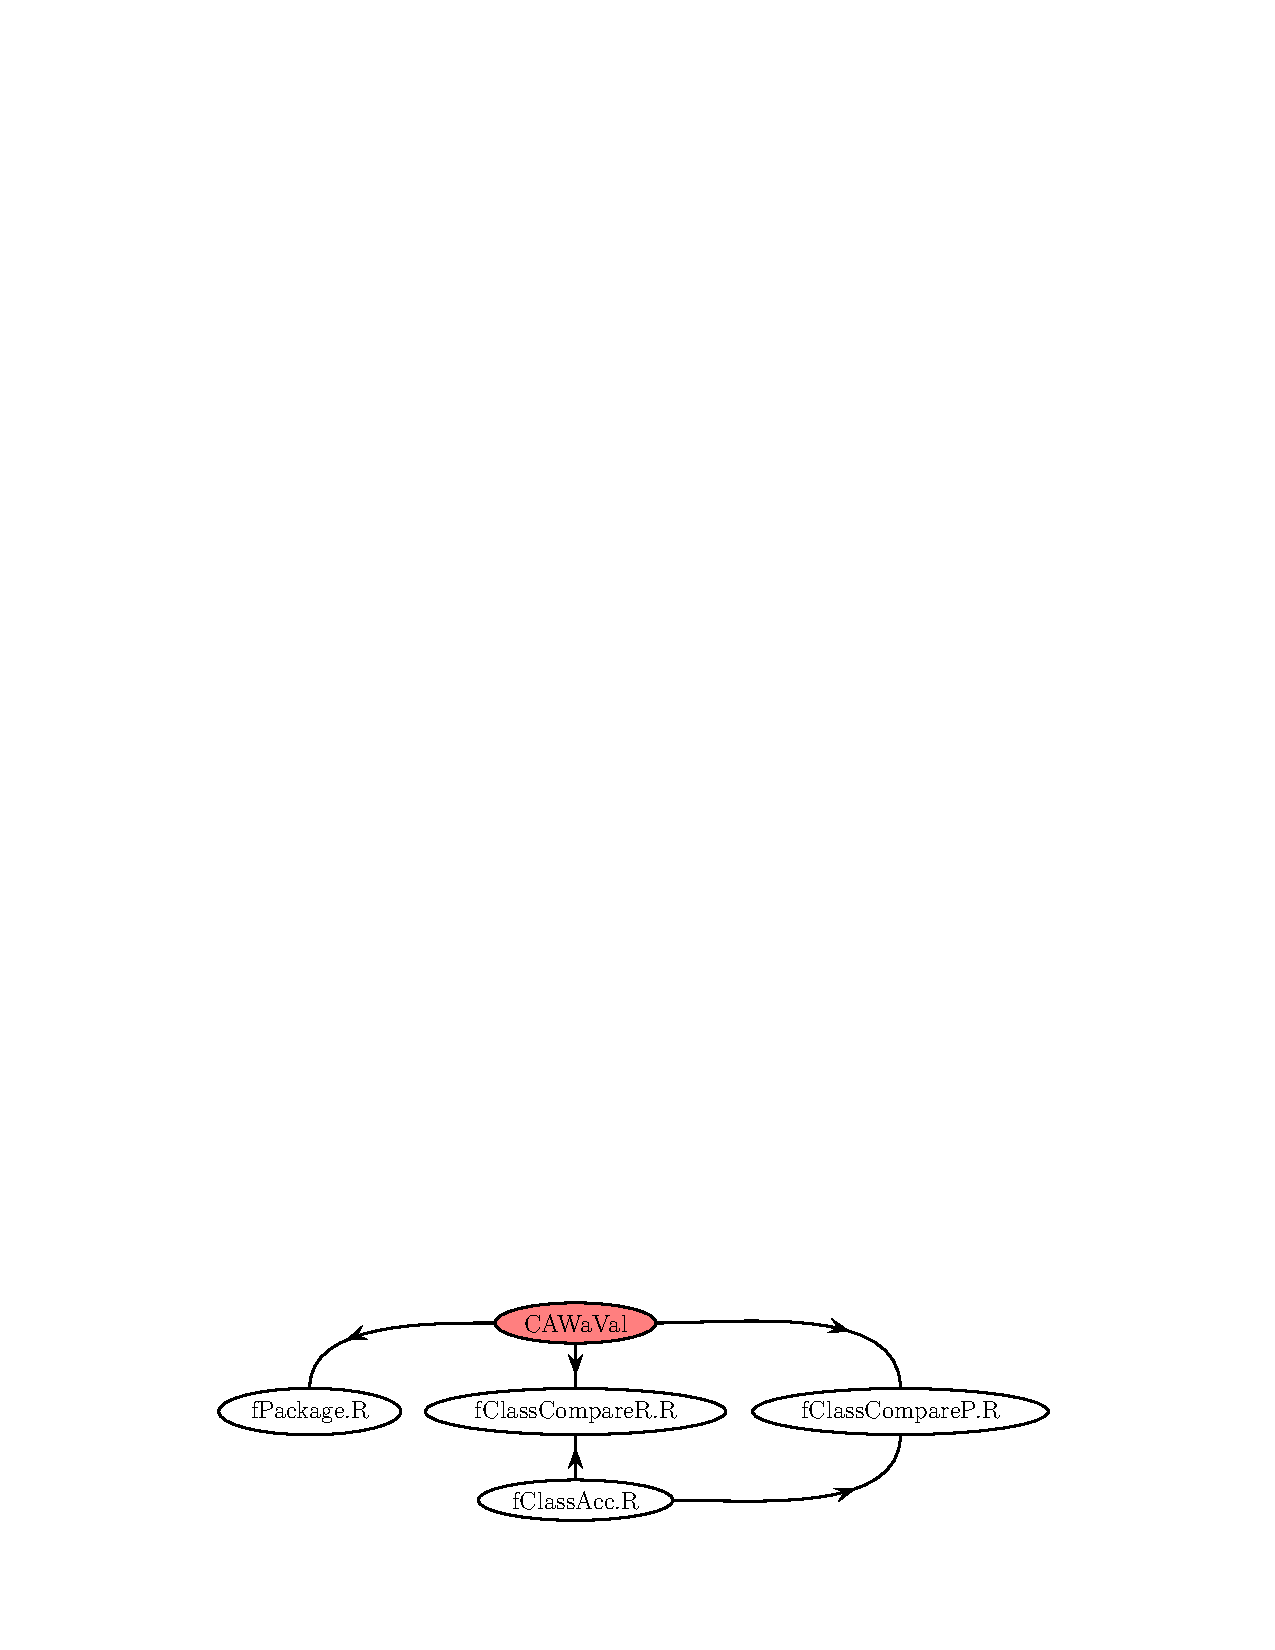
\includegraphics[width=0.75\textwidth]{figures/CAWaVal_functions.pdf}
\caption{Relations between \texttt{CAWaVal} functions.}\label{fig:cawaval-functions}
\end{figure}

\begin{table}[p]
  \centering
 \caption{\texttt{fClassCompareP}: parameters and results.}
    %\begin{tabularx}{\textwidth}{X|X}
    \begin{tabular7}{m{6.5cm}m{6.5cm}}
    \toprule
    \textbf{Parameters/results} & \textbf{Meaning} \\
    \midrule
    W.DIR & working directory \\ \midrule
    IN.DIR & directory storing input data \\ \midrule
    OUT.DIR & directory storing results \\ \midrule
    CLASS.SHP & MODIS classification result (Sec. \ref{sec:fModisClass})\\\midrule
    POINT.SHP & Point-related validation data set\\\midrule
    RASTER.FORMAT & Raster format of CLASS.RASTER\\\midrule\midrule
    $[W.DIR]/[OUT.DIR]/$ $[CLASS.SHP]\_\_[POINT.SHP]$\_AM.csv & accuracy metrics based on an overlay of CLASS.SHP and POINT.SHP\\\midrule
    $[W.DIR]/[OUT.DIR]/$ $[CLASS.SHP]\_\_[POINT.SHP]$\_CM.csv & confusion matrix based on an overlay of CLASS.SHP and POINT.SHP\\\midrule 
    $[W.DIR]/[OUT.DIR]/$ $[POINT.SHP]$\_BARPLOT.csv &  Class-specific  barplot of  samples mapped 2015 in Fergana test site.\\
    \bottomrule
    %\end{tabularx}%
    \end{tabular7}
  \label{tab:fClassCompareP}%
\end{table}


\begin{table}[p]
  \centering
  \caption{\texttt{fClassCompareR}: parameters and results.}
    %\begin{tabularx}{\textwidth}{X|X}
    \begin{tabular7}{m{6.5cm}m{6.5cm}}
    \toprule
    \textbf{Parameters/results} & \textbf{Meaning} \\
    \midrule
    W.DIR & working directory \\ \midrule
    IN.DIR & directory storing input data \\ \midrule
    OUT.DIR & directory storing results \\ \midrule
    CLASS.SHP & MODIS classification result (Sec. \ref{sec:fModisClass})\\\midrule
    CLASS.RASTER & Raster-based classification\\\midrule
    RASTER.FORMAT & Raster format of CLASS.RASTER\\\midrule\midrule
    $[W.DIR]/[OUT.DIR]/$ $[CLASS.SHP]\_\_[CLASS.RASTER]$\_AM.csv & accuracy metrics based on overlay of CLASS.SHP and CLASS.RASTER\\\midrule
    $[W.DIR]/[OUT.DIR]/$ $[CLASS.SHP]\_\_[CLASS.RASTER]$\_CM.csv & confusion matrix based on an overlay of CLASS.SHP and CLASS.RASTER\\\bottomrule
    %\end{tabularx}%
    \end{tabular7}
  \label{tab:fClassCompareR}%
\end{table}

\subsubsection{fClassCompareP}\label{sec:fClassCompareP}
The function \texttt{fClassCompareP()} combines the accuracy assessment procedure with a geometric overlay operation, where a point-related data set containing validation information is coupled with a classification result.


\begin{figure}[p]
\centering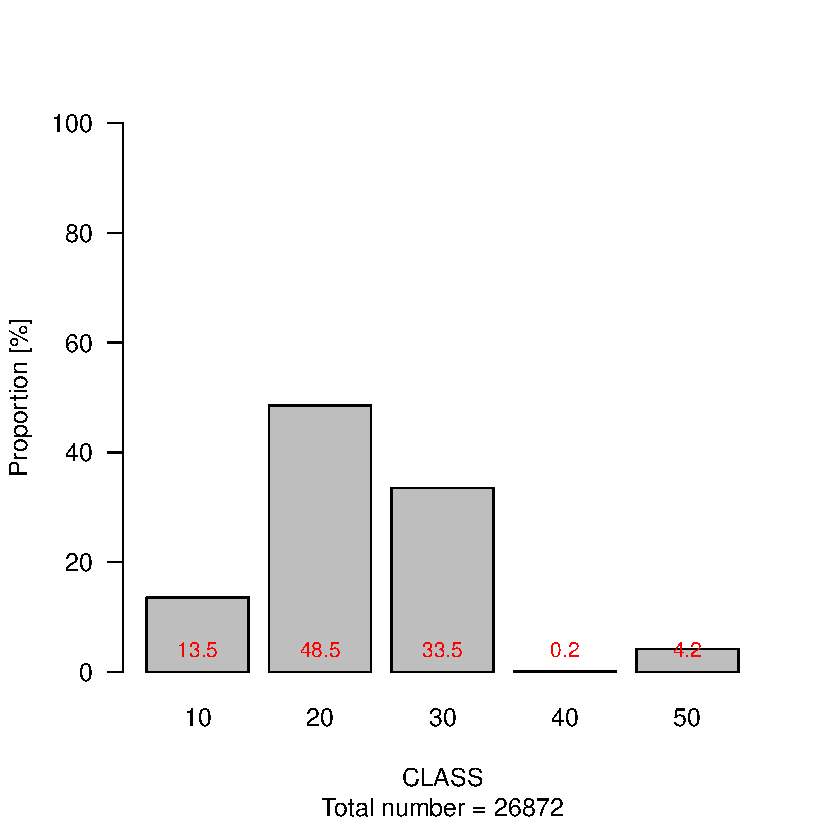
\includegraphics[width=0.55\textwidth]{figures/Fergana_2015_points_BARPLOT.pdf}
\caption{Class-specific  barplot of  samples mapped 2015 in Fergana test site.}\label{fig:fClassCompareP-barplotP}
\end{figure}

\begin{table}[p]
    \caption{\texttt{fClassCompareP} output: Confusion matrix based on an overlay of a point-related data set containing validation information and classification result for Fergana test site in 2015. 10 -- summer crop $|$ 20 -- winter crop $|$ 30 -- double crop $|$ 40 -- perennial crop $|$ 50 -- bare land.}
    \label{tab:fClassCompareP-CM}
    \centering
   \begin{tabular7}{r|r|r|r|r|r}\toprule
          & \textbf{10}    & \textbf{20}    & \textbf{30}    & \textbf{40}    & \textbf{50} \\\midrule
    \textbf{10}    & 1739  & 38    & 931   & 227   & 431 \\
    \textbf{20}    & 0     & 6341  & 2371  & 1526  & 76 \\
    \textbf{30}    & 1082  & 263   & 5021  & 1378  & 0 \\
    \textbf{40}    & 0     & 0     & 15    & 42    & 0 \\
    \textbf{50}    & 0     & 0     & 0     & 0     & 2 \\\bottomrule
    \end{tabular7}%
\end{table}

\begin{table}[p]
    \caption{\texttt{fClassCompareP} output: Accuracy metrics based on an overlay of a point-related data set containing validation information and classification result for Fergana test site in 2015. 10 -- summer crop $|$ 20 -- winter crop $|$ 30 -- double crop $|$ 40 -- perennial crop $|$ 50 -- bare land.}
    \label{tab:fClassCompareP-AM}
    \centering
       \begin{tabular7}{r|r|r|r|r|r}\toprule
          & \textbf{10}    & \textbf{20}    & \textbf{30}    & \textbf{40}    & \textbf{50} \\\midrule
   \textbf{Accuracy} & 0,61  & 0,61  & 0,61  & 0,61  & 0,61 \\\midrule
    \textbf{Precision} & 0,62  & 0,95  & 0,60  & 0,01  & 0,00 \\\midrule
    \textbf{Recall} & 0,52  & 0,61  & 0,65  & 0,74  & 1,00 \\\midrule
    \textbf{F1}    & 0,56  & 0,75  & 0,62  & 0,03  & 0,01 \\\midrule
    \textbf{Kappa} & 0,44  & 0,44  & 0,44  & 0,44  & 0,44 \\
\bottomrule
    \end{tabular7}%
\end{table}



Figure \ref{fig:fClassCompareP-barplotP} displays the barplot of samples mappped 2015 in Fergana test site. The class-specific sample numbers are quite unbalanced. This concerns especially the classes 40 (perennial crops) and 50 (bare soils), for which only few samples are available. The confusion matrix reveals, that no bare soil samples were mapped within the irrigation area during the field campaign (tab. \ref{tab:fClassCompareP-CM}). These boundary conditions also affect the accuracy metrics summarized in table \ref{tab:fClassCompareP-AM}, which show especially for the classes 40 and 50 poor results.


\subsubsection{fClassCompareR}\label{sec:fClassCompareR}
The function \texttt{fClassCompareR()} enables a validation, where a pre-classified raster data set is coupled with the MODIS classification result. The data coupling is realized by zonal statistics operations (sec. \ref{sec:ZonaSt}). In doing so, the maximum class value within each MODIS polygon is detected. Since the reference classification can be characterized by a higher geometric resolution, the range of class values is also derived. The actual accuracy assessment only considers MODIS polygones where the value range is zero.




\begin{table}[t]
    \caption{\texttt{fClassCompareR} output: Confusion matrix based on an overlay of a raster-based data set containing validation information and a classification result for the Fergana test site in 2015. 10 -- summer crop $|$ 20 -- winter crop $|$ 30 -- double crop $|$ 40 -- perennial crop $|$ 50 -- bare land.}
    \label{tab:fClassCompareR-CM}
    \centering
   \begin{tabular7}{r|r|r|r|r|r}\toprule								
          & \textbf{10} & \textbf{20} & \textbf{30} & \textbf{40} & \textbf{50} \\
    \midrule
    \textbf{10} & 533   & 0     & 6     & 2     & 169 \\
    \midrule
    \textbf{20} & 0     & 8210  & 37    & 106   & 243 \\
    \midrule
    \textbf{30} & 16    & 0     & 802   & 3     & 0 \\
    \midrule
    \textbf{40} & 13    & 38    & 40    & 1982  & 225 \\
    \midrule
    \textbf{50} & 0     & 0     & 0     & 0     & 3 \\
    \bottomrule

    \end{tabular7}%
\end{table}

\begin{table}[t]
    \caption{\texttt{fClassCompareR} output: Accuracy metrics based on an overlay of a raster-based data set containing validation information and a classification result for the Fergana test site in 2015. 10 -- summer crop $|$ 20 -- winter crop $|$ 30 -- double crop $|$ 40 -- perennial crop $|$ 50 -- bare land.}
    \label{tab:fClassCompareR-AM}
    \centering
       \begin{tabular7}{r|r|r|r|r|r}\toprule
          & \textbf{10}    & \textbf{20}    & \textbf{30}    & \textbf{40}    & \textbf{50} \\\midrule
   \textbf{Accuracy} & 0,68	& 0,68 & 0,68 & 0,68 & 0,68 \\\midrule
    \textbf{Precision} & 0,48 &	0,98 & 0,87 & 0,35 & 0,00\\\midrule
    \textbf{Recall} & 0,52  & 0,61  & 0,65  & 0,74  & 1,00 \\\midrule
    \textbf{F1}    & 0,59 &	0,97 &	0,92 &	0,50 &	0,01\\\midrule
    \textbf{Kappa} & 0,54 &	0,54 & 0,54 &	0,54 &	0,54\\\bottomrule
    \end{tabular7}%
\end{table}


For the validation of the MODIS classification from 2015, a  Landsat classification from the same year was available. Tables \ref{tab:fClassCompareR-CM} and \ref{tab:fClassCompareR-AM} provide the confusion matrix and accuracy metrics.